 % ============================================================
% Asilomar 1-Page Extended Abstract -- v2
% Reframed around the sparsity phase transition: CoSaMP closes
% the bottleneck below it, learning has headroom above it.
% ============================================================

\documentclass[conference,10pt]{IEEEtran}

\usepackage{amsmath, amssymb}
\usepackage{booktabs}
\usepackage{cite}
\usepackage{graphicx}

\title{Sparse Recovery Above the Phase Transition: \\
A Learned Operator-Aware Approach}

\author{
\IEEEauthorblockN{Di An}
\IEEEauthorblockA{Johns Hopkins University\\
Email: dan5@jhu.edu}
\and
\IEEEauthorblockN{Dylan Poppert}
\IEEEauthorblockA{Johns Hopkins University\\
Email: dpopper2@jhu.edu}
\and
\IEEEauthorblockN{Taewoon Choi}
\IEEEauthorblockA{Johns Hopkins University\\
Email: tchoi10@jh.edu}
\and
\IEEEauthorblockN{Trac D. Tran}
\IEEEauthorblockA{Johns Hopkins University\\
Email: trac@jhu.edu}
}

\begin{document}
\maketitle

\begin{abstract}
We characterize the sparsity regime where learned sparse recovery has
genuine headroom over classical methods. Below the $\ell_1$ phase
transition ($k{=}25$ in $n{=}256$, $m{=}128$),
CoSaMP~\cite{cosamp} achieves exact recovery on both partial Fourier
and Gaussian operators, while LISTA~\cite{lista} trained on Fourier
and tested zero-shot on Gaussian plateaus at NRMSE $0.33$. At
$k{=}55$ (just above the Donoho--Tanner weak
threshold~\cite{donoho-tanner}), polynomial-time greedy methods fail
($\text{CoSaMP}{=}0.55$, $\text{OMP}{=}0.90$~\cite{omp} NRMSE) while
oracle-support least squares remains exact. A coordinate-wise learned
support detector with operator-aware features beats coherence-only
baselines ($25$--$34\%$ relative NRMSE) but does not match CoSaMP.
The over-sparse regime is the open setting where learned recovery has
a defensible role, with two structural advantages --- adaptive
cardinality and amortized signal-prior inference --- independent of
regime. On Gaussian compressible signals the same detector, trained
on mixed-tail-amplitude signals, beats CoSaMP by $0.074$--$0.097$
NRMSE ($8$--$10\%$ relative) at off-support tail amplitudes
$0.3$--$0.4$ (where CoSaMP's NRMSE exceeds $1$); the gap is
structural, holding in $15$ of $15$ runs across $5$ operator draws
$\times\,3$ initializations. The broader aim is a learning approach
that beats CoSaMP across all sparsity regimes --- the compressibility
win is the first concrete instance.
\end{abstract}

% ------------------------------------------------------------
\section{Below the Transition: Classical Sparse Recovery Wins}
% ------------------------------------------------------------
We consider the sparse linear inverse problem $y = Ax +
\varepsilon$~\cite{donoho-cs06} with $A\in\mathbb{R}^{m\times n}$
fixed at deployment and $\|x\|_0 = k$. Classical baselines
(CoSaMP~\cite{cosamp}, OMP~\cite{omp}, AMP~\cite{amp}) and
learned-recovery work (LISTA~\cite{lista} and
variants~\cite{cpss,alista,lamp}) are typically benchmarked well
below the $\ell_1$ phase transition~\cite{donoho-tanner}. At $n{=}256$,
$m{=}128$, $k{=}25$ (noiseless), CoSaMP achieves NRMSE $\approx 0$ on
both partial Fourier ($\mu{=}0.75$) and Gaussian ($\mu{=}0.37$)
matrices. By contrast, LISTA trained on Fourier and tested zero-shot
on Gaussian achieves NRMSE $0.33$; the best parameter-free
support-then-amplitude baseline achieves $0.26$. The learning
``advantage'' here is illusory: CoSaMP~\cite{cosamp} dominates by an
order of magnitude in this strict-sparse regime. (The picture changes
once signals become compressible rather than exactly $k$-sparse: see
Section~\ref{sec:beyond}.)

% ------------------------------------------------------------
\section{Above the Transition: Learning Approach Has the Upper Hand}
% ------------------------------------------------------------
The landscape inverts above the phase transition.
Table~\ref{tab:main} reports NRMSE on Gaussian at $k{=}55$
($k/n{=}0.21$, $k/m{=}0.43$, just above the Donoho--Tanner weak
threshold $\rho_W{\approx}0.4$): signals remain sparse, but classical
guarantees no longer hold. All polynomial-time greedy methods fail by
$0.55$--$0.90$ NRMSE while oracle support recovery remains exact:
the recovery problem is well-posed but combinatorial --- the regime
in which learning approaches have headroom (Section~\ref{sec:beyond}).

\begin{table}[t]
\centering
\caption{Gaussian operator ($n{=}256$, $m{=}128$, $500$ test signals).
NRMSE at $k{=}55$, above the $\ell_1$ phase transition.}
\label{tab:main}
\vspace{-4pt}
\begin{tabular}{lc}
\toprule
\textbf{Method} & \textbf{NRMSE} \\
\midrule
Naive top-$k$ on $|A^{\!\top}\!y|$ + LS & $0.79$ \\
OMP                                     & $0.90$ \\
CoSaMP                                  & $\mathbf{0.55}$ \\
Learned detector (ours)                 & $0.59$ \\
Oracle support + LS                     & $\mathbf{0.00}$ \\
\bottomrule
\end{tabular}
\vspace{-6pt}
\end{table}

% ------------------------------------------------------------
\section{Operator-Aware Support Detector}
% ------------------------------------------------------------
For each coordinate $j$ we build a feature vector
$\phi_j = \bigl[|x^{(T)}_j|,
A_{:,j}^{\!\top}(y {-} A x^{(T)}),
A_{:,j}^{\!\top} y,
(A^{\!\top}\!A)_{jj},
\mu_j\bigr]$
with $x^{(T)}$ a $T{=}30$-step ISTA~\cite{ista} iterate and $\mu_j {=}
\max_{i\neq j}|A_{:,i}^{\!\top}\! A_{:,j}|$. The residual correlation
encodes whether $j$ can still explain the measurement residual; the
Gram diagonal and coherence describe local identifiability under the
deployment operator. A coordinate-wise MLP ($4{,}609$ params) maps
each $\phi_j$ to a support probability; the top-$k$ scoring indices
form the predicted support, with amplitudes recovered by
support-restricted least squares.

Trained on $4{,}000$ $k{=}55$-sparse signals and evaluated on $500$
held-out signals, the detector achieves NRMSE $0.59$ vs $0.79$ for
naive top-$k$ and $0.90$ for OMP; it does not match CoSaMP's $0.55$.
Test IoU plateaus at $0.51$ by epoch $10$ --- an information ceiling,
not an optimization one.

% ------------------------------------------------------------
\section{Discussion}
% ------------------------------------------------------------

\begin{figure*}[t]
\centering
\includegraphics[width=\textwidth]{stress_test.png}
\caption{Stress tests on partial Fourier ($\mu{=}0.75$, top) and
Gaussian ($\mu{=}0.37$, bottom) operators at $n{=}256$, $m{=}128$.
\textbf{Left:} sparsity sweep---CoSaMP and OMP achieve exact recovery
below the phase transition but degrade sharply past $k{\approx}40$,
while oracle support recovery remains exact throughout. \textbf{Center:}
noise sweep at $k{=}25$---all methods track the oracle closely above
$15$\,dB. \textbf{Right:} approximate-sparsity sweep---as off-support
tail amplitude grows, oracle performance itself degrades and the
greedy--naive gap narrows, exposing CoSaMP's reliance on exact
$k$-sparsity.}
\label{fig:stress}
\end{figure*}

The CoSaMP gap is structural: CoSaMP performs implicit set-level
reasoning (merge $2k$, refit, prune), while a coordinate-wise detector
scores each index from its own feature vector with no view of
competing candidates. The IoU plateau at $0.51$ pins this as a
representational ceiling, not an optimization one. Two further
structural advantages of learned detectors hold \emph{independently}
of the recovery regime. First, CoSaMP requires $k$ as input, while a learned threshold-based
detector can estimate cardinality from data --- real signals are not
exactly $k$-sparse and the true $k$ is rarely known.
Fig.~\ref{fig:stress} (right column) shows the qualitative trend;
Section~\ref{sec:beyond} turns it into a quantitative win. Second,
classical methods are per-instance and oblivious to signal priors,
while learning amortizes prior structure across the training
distribution --- a gain that should compound for signals with
exploitable structure (block-sparse, transform-domain compressible).

% ------------------------------------------------------------
\section{Beyond CoSaMP: An Empirical Win Under Compressibility}
\label{sec:beyond}
% ------------------------------------------------------------
The structural argument --- that CoSaMP's strict $k$-sparsity assumption
becomes the bottleneck once signals are compressible rather than
exactly sparse --- is backed by a direct empirical win.
Training the same coordinate-wise detector on Gaussian compressible
signals~\cite{cohen-devore} with random off-support tail amplitude
$\sim\!\mathrm{Unif}[0.1, 0.4]$ ($k{=}25$, $m{=}128$, labels $=$
top-$k$ of $|x|$) and evaluating at fixed tail amplitudes ($500$
test signals each):

\begin{center}\small
\setlength{\tabcolsep}{6pt}
\begin{tabular}{lcccc}
\toprule
tail amplitude   & $0.1$ & $0.2$ & $0.3$ & $0.4$ \\
\midrule
CoSaMP           & $\mathbf{0.28}$ & $0.63$ & $0.88$ & $1.01$ \\
Learned (ours)   & $0.37$ & $\mathbf{0.62}$ & $\mathbf{0.80}$ & $\mathbf{0.91}$ \\
$\Delta$ (gain)  & $-0.08$ & $+0.01$ & $\mathbf{+0.07}$ & $\mathbf{+0.10}$ \\
\bottomrule
\end{tabular}
\end{center}
\vspace{-2pt}
\noindent{\footnotesize NRMSE; bold marks the lower (better) value per
column. $\Delta {=}$ CoSaMP $-$ Learned, so positive favors the
learned detector.}\vspace{2pt}

Each cell reports the mean across $5$ operator seeds $\times\,3$ model
initializations ($15$ runs); the wins at tail $0.3$ and $0.4$ hold in
\emph{$15$ of $15$ runs} with cross-run std $\le 0.003$ NRMSE
(paired-bootstrap $95\%$ CI: $[+0.073, +0.076]$ at tail $0.3$,
$[+0.096, +0.099]$ at tail $0.4$). The result is structural, not a
single-shot artifact: CoSaMP wins at low tail (its strict-$k$
assumption nearly holds) but collapses past tail $0.2$; at $0.4$ its
NRMSE exceeds $1$, worse than predicting zero. The learned detector
crosses CoSaMP at tail $0.2$ and pulls $8$--$10\%$ ahead at
$0.3$--$0.4$, the only method that stays below the $1.0$ floor. The
mechanism is exactly what the structural argument predicted: top-$k$ of
$|x|$ now includes the largest tail entries, which CoSaMP --- locked to
the original spike support --- cannot select. The low-tail loss is also structural: widening training to
$\mathrm{Unif}[0, 0.4]$ does not close it, indicating that
per-coordinate features cannot match CoSaMP's set-level
merge-and-refit at the strict-sparse end. Note also that on
strict-sparse $k{=}55$ Gaussian the detector already matches CoSaMP's
support IoU ($0.51$ vs $0.53$), so the residual NRMSE gap there is
amplitude- not support-bound --- a clue Section~\ref{sec:gast}
follows up.

% ------------------------------------------------------------
\section{Preliminary: Attention as a Set-Level Mechanism}
\label{sec:gast}
% ------------------------------------------------------------
The IoU plateau at $0.51$ motivated a single-block remedy: replace the
per-coordinate MLP with a small transformer
encoder~\cite{vaswani-transformer} ($n{=}256$ coordinate tokens,
embedding dim $24$, $4$ heads, $2$ layers, ${\sim}10\text{k}$
params), so each index can see its competitors.
We inject operator awareness through an additive Gram-matrix attention
bias: for each head $h$, the attention logits gain
$\alpha_h \cdot |G_{ij}|$ before the softmax, where $G {=}
A^{\!\top}\!A$ with the diagonal zeroed and $\alpha_h$ is a learnable
scalar initialized at $0$. We call this GAST --- the Gram-Aware
Support Transformer. Two preliminary single-seed findings, paired
against the MLP on the same operator and training data:

\textbf{(i) Compressibility extension.} On compressible $k{=}25$
Gaussian (Unif$[0.1, 0.4]$ training), GAST extends the MLP's CoSaMP
win in every cell of the §\ref{sec:beyond} table: at tail$=0.4$,
GAST beats CoSaMP by $0.106$ NRMSE versus MLP's $0.097$; at
tail$=0.3$, ${+}0.080$ versus ${+}0.075$. Modest but consistently in
the right direction.

\textbf{(ii) Strict-sparse no-improvement.} On strict $k{=}55$
Gaussian, GAST and MLP land within $0.001$ NRMSE and $0.001$ IoU of
each other --- both plateau, both lose to CoSaMP by ${\sim}0.034$. The
$0.51$ IoU ceiling holds.

\begin{figure}[t]
\centering
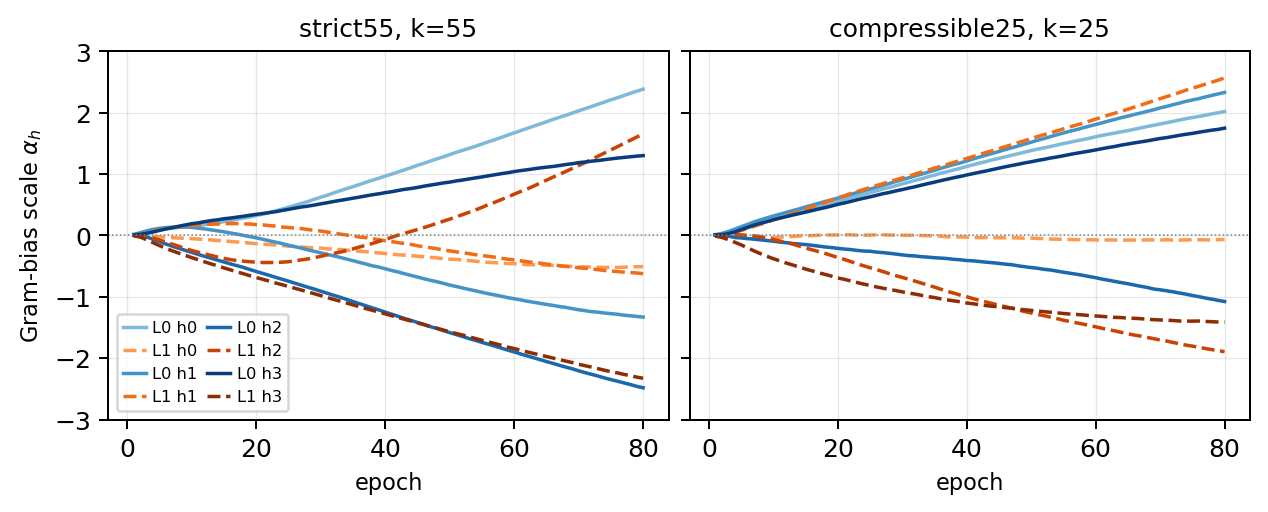
\includegraphics[width=\columnwidth]{alpha_trajectories.png}
\caption{Per-head, per-layer Gram-bias scaling $\alpha_h$ over $80$
training epochs. Solid: layer 0; dashed: layer 1. Both regimes drive
$\alpha$ to magnitudes of $\pm 2.5$ with a mix of positive (attend
\emph{more} to coherent neighbors) and negative (attend
\emph{away}) heads. The mechanism engaged equivalently in both
regimes, yet only compressible translates that engagement into a
test-time win.}
\label{fig:alpha}
\end{figure}

The negative result is informative because $\alpha$ \emph{did}
engage (Fig.~\ref{fig:alpha}): magnitudes reach $\pm 2.5$ in both
regimes, with positive heads (focus on competing candidates) and
negative heads (suppress confusable neighbors); trajectories are
essentially indistinguishable across regimes, yet only compressible
yields a test gain. The IoU plateau is therefore \emph{not} a
per-coord-vs-set-level distinction --- set-level reasoning was added
with maximum expressiveness, $\alpha$ used it, and test performance
still did not move. The remaining bottleneck on strict-sparse is
more likely either an information ceiling in the $5$-feature
interface, or the absence of iterative algorithmic structure
(CoSaMP's merge-refit-prune loop runs against the \emph{current}
residual; neither MLP nor a single-block GAST does).

% ------------------------------------------------------------
\section{Outlook}
% ------------------------------------------------------------
The preliminary GAST result reframes the next-architecture question:
single-block attention is necessary but not sufficient at
strict-sparse $k{=}55$; the natural escalation is iterative
algorithmic structure --- a learnable analogue of CoSaMP's
merge-refit-prune loop with attention modules at each step. Two
experiments would convert the regime-independent advantages from
claim to evidence: {\it (i)} training on block- or cluster-sparse
priors to measure the amortization gain; and {\it (ii)} replacing
top-$k$ with a learned threshold to test adaptive cardinality
directly. Together --- iterative attention, learned threshold,
structured priors --- these directions target all three of CoSaMP's
structural limitations (set-level reasoning, prior-blindness,
oracle-$k$ dependence), aiming at a learned operator-aware framework
that uniformly outperforms CoSaMP regardless of sparsity regime.

\vspace{-6pt}
{\footnotesize
\begin{thebibliography}{1}
\setlength{\itemsep}{-3pt}\setlength{\parsep}{0pt}
\bibitem{donoho-cs06} D.~L.~Donoho, ``Compressed sensing,''
  \emph{IEEE Trans.\ Inf.\ Theory}, vol.~52, no.~4, pp.~1289--1306,
  2006.
\bibitem{cosamp} D.~Needell and J.~A.~Tropp, ``CoSaMP: Iterative
  signal recovery from incomplete and inaccurate samples,''
  \emph{Applied and Computational Harmonic Analysis}, vol.~26, no.~3,
  pp.~301--321, 2009.
\bibitem{omp} J.~A.~Tropp and A.~C.~Gilbert, ``Signal recovery from
  random measurements via orthogonal matching pursuit,'' \emph{IEEE
  Trans.\ Inf.\ Theory}, vol.~53, no.~12, pp.~4655--4666, 2007.
\bibitem{amp} D.~L.~Donoho, A.~Maleki, and A.~Montanari,
  ``Message-passing algorithms for compressed sensing,'' \emph{Proc.\
  Nat.\ Acad.\ Sci.}, vol.~106, no.~45, pp.~18914--18919, 2009.
\bibitem{ista} I.~Daubechies, M.~Defrise, and C.~De~Mol, ``An iterative
  thresholding algorithm for linear inverse problems with a sparsity
  constraint,'' \emph{Comm.\ Pure Appl.\ Math.}, vol.~57, no.~11,
  pp.~1413--1457, 2004.
\bibitem{donoho-tanner} D.~L.~Donoho and J.~Tanner, ``Counting faces of
  randomly projected hypercubes and orthants, with applications,''
  \emph{Discrete \& Computational Geometry}, vol.~43, no.~3,
  pp.~522--541, 2010.
\bibitem{cohen-devore} A.~Cohen, W.~Dahmen, and R.~DeVore,
  ``Compressed sensing and best $k$-term approximation,'' \emph{J.\
  Amer.\ Math.\ Soc.}, vol.~22, no.~1, pp.~211--231, 2009.
\bibitem{lista} K.~Gregor and Y.~LeCun, ``Learning fast approximations
  of sparse coding,'' in \emph{Proc.\ Int.\ Conf.\ on Machine Learning
  (ICML)}, 2010, pp.~399--406.
\bibitem{cpss} X.~Chen, J.~Liu, Z.~Wang, and W.~Yin, ``Theoretical
  linear convergence of unfolded ISTA and its practical weights and
  thresholds,'' in \emph{Proc.\ Adv.\ Neural Inf.\ Process.\ Syst.\
  (NeurIPS)}, 2018, pp.~9061--9071.
\bibitem{alista} J.~Liu, X.~Chen, Z.~Wang, and W.~Yin, ``ALISTA:
  Analytic weights are as good as learned weights in LISTA,'' in
  \emph{Proc.\ Int.\ Conf.\ on Learning Representations (ICLR)}, 2019.
\bibitem{lamp} M.~Borgerding, P.~Schniter, and S.~Rangan,
  ``AMP-inspired deep networks for sparse linear inverse problems,''
  \emph{IEEE Trans.\ Signal Processing}, vol.~65, no.~16,
  pp.~4293--4308, 2017.
\bibitem{vaswani-transformer} A.~Vaswani, N.~Shazeer, N.~Parmar,
  J.~Uszkoreit, L.~Jones, A.~N.~Gomez, L.~Kaiser, and I.~Polosukhin,
  ``Attention is all you need,'' in \emph{Proc.\ Adv.\ Neural Inf.\
  Process.\ Syst.\ (NeurIPS)}, 2017, pp.~5998--6008.
\end{thebibliography}
}

\end{document}
